 
\chapter{工具变量的计量经济学视角}
 \label{chapter::iv-econometric}
 
 
第\ref{chapter::iv-experiment}章与第\ref{chapter::iv-inequalities}章从实验角度探讨了工具变量法。图\ref{fig::causal-diagram-IV}则直观展示了这一方法的理论依据。 
 
 
\begin{figure}[h]
\centering 
$
\xymatrix{
 && & U  \ar[dl] \ar[dr] &\\
Z \ar[rr] &&D \ar[rr]&&Y
}
$
\caption{工具变量的因果图}\label{fig::causal-diagram-IV}
\end{figure} 
 
 
 
在存在不依从的鼓励设计中，$Z$经过随机化，因此与实际接受处理$D$和结果$Y$之间的混杂变量$U$独立。处理分配$Z$对结果$Y$没有直接效应，而只经由实际接受处理$D$影响结果$Y$，因而充当$D$的工具变量。这里的工具变量由实验者产生。 


许多应用无法随机化。若处理$D$与结果$Y$之间存在未测量混杂，应如何作因果推断？计量经济学的一个巧妙想法是寻找{\it 自然实验}，模拟鼓励设计。为识别$D$对$Y$的因果效应，可寻找另一个变量$Z$，使其满足图\ref{fig::causal-diagram-IV}编码的假设。变量$Z$必须满足以下条件：
\begin{enumerate}
\item
近似具备随机化特性，从而与未观测混淆因素$U$独立；
\item
能够改变治疗干预$D$的分布规律；
\item
它只能通过$D$间接影响结果$Y$，不能直接影响结果。
\end{enumerate}
若上述条件均被满足，则$Z$便可作为估计$D$对$Y$影响程度的有效工具变量。 



本章介绍基于线性回归的传统计量经济学工具变量视角。\citet{imbens1994identification}与\citet{angrist1996identification}澄清了这一视角与第\ref{chapter::iv-experiment}、\ref{chapter::iv-inequalities}章实验视角之间的联系，是一项基础性贡献。下面先看例子，再讨论代数细节。 



\section{工具变量法的实证研究案例}
 
 
 
寻找合适的工具变量与其说是科学，不如说是一门艺术。尽管后文涉及的代数运算在统计学中并不算复杂，但如何在实证研究中精准找到符合要求工具变量却极具挑战性。以下列举若干典型实例。  


\begin{example} 
鼓励设计中，$Z$是随机分配的处理，$D$是最终接受的处理，$Y$是结果。如第\ref{chapter::iv-experiment}章所述，图\ref{fig::causal-diagram-IV}的工具变量假设在双盲随机对照试验中较为合理，这是工具变量的理想情形。 
\end{example}


 
 
 \begin{example}
 \citet{hearst1986delayed}发现越战征兵抽签中号码较小的男性随后死亡率较高；其解释为兵役产生的负面影响。\citet{angrist1990lifetime}补充指出这类男性后期收入也偏低，同样可归结为兵役所致。由于抽签号码属随机生成、号码较小者恰更可能服兵役，且该号码对死亡率与收入并无直接影响，故图\ref{fig::causal-diagram-IV}条件完全成立。\citet{angrist1996identification}正是以此为基础重新分析了实验数据：其中抽签号码为工具变量、兵役为处理干预、死亡率或收入则为观测结果。 
\end{example}




\begin{example}
\citet{angrist1991does}以出生季度作为工具变量，测算了受教育年限对收入的贡献值。出生季度具有近似随机化特征：一方面美国多数州规定儿童满六周岁方可入学；另一方面义务教育法要求最低入学年龄为十六周岁。此外出生季度亦不直接影响收入值。 
\end{example}


\begin{example}
\citet{angrist1998children}选用兄弟姐妹性别构成作为工具变量，研究了家庭规模对母亲劳动参与的影响。同理，此变量亦具备近似随机化特征：同性别双胞胎会显著提升第三胎仍为同性别的概率，且该变量同样不直接决定母亲的就业行为。 
\end{example}


\begin{example}\label{example::Card1993}
\citet{card1993using}研究教育对工资的影响，以居住地点距大学远近的地理差异作为工具变量。具体而言，$Z$包含是否在两年制或四年制大学附近长大的虚拟变量。尽管该研究很经典，它未必是一个理想的工具变量例子：父母选择住址可能并非随机，而且成长地点本身也可能影响后来工资。 
\end{example}



\begin{example}
\citet{voight2012plasma}用{\it 孟德尔随机化}研究血浆高密度脂蛋白（HDL）胆固醇对心肌梗死风险的因果效应。他们采用某些单核苷酸多态性（SNP）作为 HDL 的遗传工具变量：依据孟德尔第二定律，它们与 HDL 和心肌梗死之间的未测量混杂独立，且仅通过 HDL 影响心肌梗死。孟德尔随机化的更多细节见第\ref{chapter::iv-mr}章。 
\end{example}



\section{普通最小二乘法简述}



在引入工具变量法前，我们先简要回顾普通最小二乘法（见\ref{appendix::basic-linear-regression}章）。该方法是统计学经典内容，但其数学定义形式各异，且不同形式间的选择将影响理论解释。 

第一种视角基于投影。给定具有有限二阶矩的随机变量$Y$与随机变量或向量$D$，定义总体 OLS 系数
\begin{eqnarray*}
\beta  &=& \arg\min_b E(Y - D  \tran b  )^2 \\
&=& E(DD\tran)^{-1} E(DY),
\end{eqnarray*}
再定义总体残差$\varepsilon = Y -  D  \tran \beta $。根据定义，$Y$可分解为
\begin{eqnarray}\label{eq::olsdecomposition}
Y = D  \tran \beta  + \varepsilon,
\end{eqnarray}
且必满足
$$
E(  D \varepsilon) = 0.
$$
根据数据$(D_i,Y_i)_{i=1}^n \iidsim (D, Y)$，$\beta$的 OLS 估计是矩估计量
$$
\hat{\beta} = \left(  \sumn D_i D_i\tran \right)^{-1}   \sumn D_i Y_i  . 
$$
由于
\begin{eqnarray*}
\hat{\beta}  &=& \left(  \sumn D_i D_i\tran \right)^{-1}  \sumn D_i ( D_i\tran \beta + \varepsilon_i   )  \\
&=& \beta + \left(  \sumn D_i D_i\tran \right)^{-1} \sumn D_i  \varepsilon_i   ,
\end{eqnarray*}
利用大数定律和$E(\varepsilon D) = 0.$，可证明$\hat{\beta}$一致估计$\beta$。$\cov(\hat\beta)$的经典 EHW 稳健方差估计为
$$
\hat{V}_\textsc{ehw} = \left(  \sumn D_i D_i\tran \right)^{-1}
\left(  \sumn \hat{\varepsilon}_i^2 D_i D_i\tran \right)
\left(  \sumn D_i D_i\tran \right)^{-1}
$$
其中$\hat{\varepsilon}_i  = Y_i - D_i\tran \hat{\beta}$是残差。 




第二种视角把
\begin{eqnarray}\label{eq::ols-true-model}
Y = D  \tran \beta  + \varepsilon,
\end{eqnarray}
视为数据生成过程的真实模型：给定随机变量$(D, \varepsilon)$，根据线性方程\eqref{eq::ols-true-model}生成$Y$。在这一生成过程中，$\varepsilon$与$D$可能相关，即$E( D \varepsilon) \neq  0$，图\ref{fig::endogenous-regressor}就是例子。这与第一种视角有根本区别：第一种视角中的$E(\varepsilon D) = 0$由总体 OLS 的定义自动保证。因此，当样本量$n$趋于无穷时，OLS 估计量可能不一致：
$$
\hat{\beta} \rightarrow \beta + E(DD\tran)^{-1} E(D\varepsilon) \neq \beta 
$$
这里为依概率收敛。 


本节最后根据\eqref{eq::ols-true-model}定义{\it 内生}与{\it 外生}回归变量，不过这些术语在计量经济学中并非只有一种定义。 



\begin{definition}
\label{def::endogenous-exogenous}
当$E(\varepsilon D) \neq  0$时，回归变量$D$称为{\it 内生的}；当$E(\varepsilon D) =  0$时，回归变量$D$称为{\it 外生的}。 
\end{definition}

定义\ref{def::endogenous-exogenous}采用计量经济学的标准术语。$E(\varepsilon D) \neq  0$时，也称存在{\it 内生性}；$E(\varepsilon D) =  0$时，也称满足{\it 外生性}。

在第一种最小二乘视角下，由于$E(\varepsilon D) =  0$为定义前提，内生与外生的区分毫无意义。持此观点的统计学家常觉这两概念难以理解，进而难以接受工具变量的必要性。若要深入理解工具变量法，必须转而采用第二种视角。 




 

\begin{figure}[h]
\centering
\begin{subfigure}[]{0.4\textwidth}
                \centering
$
\xymatrix{
& U \ar[dl] \ar[dr]& \\
D \ar[dr] & & \varepsilon \ar[dl] \\
&Y&
}
$                \caption{$E(D\varepsilon) \neq 0$}
        \end{subfigure}%
        
        \begin{subfigure}[]{0.4\textwidth}
                \centering
$
\xymatrix{
&\varepsilon  \ar[dl] \ar[dr] &\\
D \ar[rr]&&Y
}
$
                \caption{对$\varepsilon$边际化处理}
        \end{subfigure}%
        
\caption{内生变量$D$的不同表现形式。上图中$U$代表$D$与$\varepsilon$共享的未观测混淆因素。}\label{fig::endogenous-regressor}
\end{figure}



\section{线性工具变量模型}
\label{sec::linear-iv-model}



$D$内生时，OLS 估计不一致，必须利用额外信息才能构造$\beta$的一致估计量。下面关注如下线性工具变量模型：


\begin{definition}
[线性工具变量模型]\label{def::linear-iv-model}
定义观测模型为
$$
Y = D  \tran \beta  + \varepsilon ,
$$
且须满足
\begin{eqnarray}\label{eq::iv-moment-condition}
E(\varepsilon Z) = 0 . 
\end{eqnarray}
\end{definition}


定义\ref{def::linear-iv-model}的线性工具变量模型可用下列因果图表示： 
%\begin{figure}[h]
%\centering 
$$
\xymatrix{
&&&\varepsilon  \ar[dl] \ar[dr] &\\
Z\ar[rr]&&D \ar[rr]&&Y
}
$$
%\caption{Instrumental variable}
%\end{figure}

上述模型虽然允许$E(\varepsilon D) \neq 0$，却提出了额外矩条件\eqref{eq::iv-moment-condition}。通过加入截距项使$E(\varepsilon) = 0$后，此条件可解读为$Z$与误差项$\varepsilon$不相关。但任何随机噪声均与$\varepsilon$不相关，故必须补充条件确保$Z$对估计$\beta$切实有效。直观而言，该条件要求$Z$须与$D$存在相关性——具体技术细节下文详述。  
 

数学条件\eqref{eq::iv-moment-condition}看似简单，但实证研究的一项核心挑战，正是找到满足\eqref{eq::iv-moment-condition}的变量$Z$。条件\eqref{eq::iv-moment-condition}涉及不可观测的$\varepsilon$，因此一般无法检验。 
 


\section{恰好识别情形}
\label{sec::iv-just-identify}

我们先探讨$Z$与$D$维度相同且$E(ZD\tran)$满秩的特殊情形。此时条件$E(\varepsilon Z) = 0$等价于
$$
E\{  Z (Y -  D \tran \beta) \} = 0 .
$$
解此线性系统可得
$$
E(  ZY)  = E(ZD\tran) \beta  \\
 \Longrightarrow 
\beta = E(ZD\tran) ^{-1} E(  ZY)  
$$
前提是$E(ZD\tran)$非退化矩阵。当$E(\varepsilon D) = 0$时，即$D$本身充当工具变量，此式即退化为普通最小二乘估计量：
\begin{eqnarray}\label{eq::iv-estimator}
\hat{\beta}_\textsc{iv} = \left(  \sumn Z_i D_i\tran \right)^{-1}  \sumn Z_iY_i.
\end{eqnarray}

将$D$与$Z$都为标量的情形具体推导出来有助于理解，见下面的例\ref{eg::scalar-iv}。

\begin{example}\label{eg::scalar-iv}
在含截距、$D$与$Z$均为标量的简单情形中，模型为
$$
\left\{ \begin{array}{l}
Y = \alpha +  \beta  D + \varepsilon ,\\
E(\varepsilon) = 0, \quad \cov(\varepsilon, Z) = 0,
\end{array}
\right.
$$
由该模型，
$$
\cov( Z, Y ) = \beta \cov(Z, D) 
$$
因而
$$
 \beta = \frac{ \cov( Z, Y )   }{ \cov(Z, D) }.
$$
将分子分母同时除以$\var(Z)$，得到
$$
\beta =  \frac{ \cov( Z, Y ) / \var(Z)  }{ \cov(Z, D) / \var(Z) },
$$
即$Y$和$D$分别对$Z$作 OLS 回归所得$Z$系数之比。若$Z$为二元变量，这两个系数就是均值差（见习题\ref{problem::pols-binary}），$\beta$简化为
$$
\beta = \frac{ E(Y\mid Z=1) - E(Y\mid Z=0)  }{ E(D\mid Z=1) - E(D\mid Z=0) } .
$$
与定理\ref{thm::CACE-identification}的识别公式相同。也就是说，对于二元工具变量$Z$和二元处理$D$，工具变量估计在潜在结果框架下恢复 CACE。这是\citet{imbens1994identification}与\citet{angrist1996identification}的关键结论。  
\end{example}



 

\section{过度识别情形}
\label{sec::sec::iv-over-identify}

第\ref{sec::iv-just-identify}节讨论的是{\it 恰好识别}情形。若$Z$的维数小于$D$，且$E(ZD\tran)$不满列秩，则方程$E(  ZY)  = E(ZD\tran) \beta$有无穷多个解。这就是{\it 欠识别}：即使有$Z$，也无法唯一确定系数$\beta$。这一困难问题超出本书范围。为保证可识别性，工具变量数至少应与内生回归变量数一样多。 

若$Z$的维数大于$D$，且$E(ZD\tran)$满列秩，就有多种办法根据$E(  ZY)  = E(ZD\tran) \beta$确定$\beta$。而且，样本对应方程
$$
n^{-1} \sumn Z_iY_i = n^{-1} \sumn Z_i D_i\tran \beta
$$
的方程数多于未知参数数，可能没有精确解。 


处理过度识别的一种巧妙计算方法是{\it 两阶段最小二乘}（TSLS）估计量\citep{theil1953estimation, basmann1957generalized}，它分两步进行。

\begin{definition}
[两阶段最小二乘法]\label{def::2sls}
以$Z$为工具变量的$D$系数的 TSLS 估计量定义如下。 
\begin{enumerate}
\item
将$D$对$Z$作 OLS 回归，得到拟合值$\hat{D}_i\ (i=1,\ldots, n)$。若$D_i$为向量，则逐分量回归以获得$\hat{D}_i$。将拟合向量按行$\hat{D}_i\tran $组成矩阵$\hat{D}$；
\item
以$\hat{D}$为自变量回归$Y$，所得斜率系数即为$\hat{\beta}_\textsc{tsls}$值。  
\end{enumerate}
\end{definition}
 

为说明 TSLS 为什么有效，需要进一步的代数推导。将其明确写为
\begin{eqnarray} 
\hat{\beta}_\textsc{tsls} &=& \left(  \sumn \hat{D}_i\hat{D}_i\tran \right) ^{-1} 
\sumn \hat{D}_i Y_i  \label{eq::2sls-definition} \\
&=& \left(  \sumn \hat{D}_i\hat{D}_i\tran \right) ^{-1} 
\sumn \hat{D}_i (D_i \tran \beta + \varepsilon_i)  \nonumber  \\
&=& \left(  \sumn \hat{D}_i\hat{D}_i\tran \right) ^{-1} 
\sumn \hat{D}_i D_i \tran \beta + \left(  \sumn \hat{D}_i\hat{D}_i\tran \right) ^{-1} \sumn \hat{D}_i  \varepsilon_i .   \nonumber 
\end{eqnarray}
第一阶段 OLS 保证$D_i  = \hat{D}_i + \check D_i$，且拟合值与残差正交，即
\begin{equation} \label{eq::ols-orthogonal}
\sumn \hat{D}_i  \check D_i\tran = 0
\end{equation}
是与$D_i$维数相同的零方阵。正交关系\eqref{eq::ols-orthogonal}蕴含
$$
\sumn \hat{D}_i D_i \tran = \sumn \hat{D}_i\hat{D}_i\tran,
$$
从而
\begin{eqnarray}
\label{eq::2sls-ols}
\hat{\beta}_\textsc{tsls} = \beta + \left(  \sumn \hat{D}_i\hat{D}_i\tran \right) ^{-1} \sumn \hat{D}_i  \varepsilon_i.
\end{eqnarray}
第一阶段 OLS 还保证
\begin{equation}
\label{eq::ols-donz}
\hat{D}_i = \hat{\Gamma}\tran  Z_i 
\end{equation}
进而
\begin{eqnarray}
\label{eq::2sls-consistency}
\hat{\beta}_\textsc{tsls} = \beta + \left\{  \hat{\Gamma}\tran  \left(  n^{-1}  \sumn Z_i Z_i\tran  \right) \hat{\Gamma}  \right\}  ^{-1}  
\hat{\Gamma}\tran  \left( n^{-1} \sumn Z_i  \varepsilon_i \right) . 
\end{eqnarray}
由\eqref{eq::2sls-consistency}，利用大数定律以及$n^{-1} \sumn Z_i  \varepsilon_i $的概率极限为$E(Z\varepsilon) = 0$，即可得到 TSLS 的一致性。还可利用\eqref{eq::2sls-consistency}证明：$Z$与$D$维数相同时，$\hat{\beta}_\textsc{tsls} $与第\ref{sec::iv-just-identify}节定义的$\hat{\beta}_\textsc{iv} $在数值上相同，见习题\ref{prob::algebra-tsls}。 




根据\eqref{eq::2sls-ols}，标准误可按以下方式计算：先求残差$\hat{\varepsilon}_i = Y_i - \hat{\beta}_\textsc{tsls}\tran D_i$，再计算稳健方差估计
$$
\hat{V}_\textsc{tsls} = \left( \sumn  \hat{D}_i \hat{D}_i\tran  \right)^{-1}
 \left( \sumn \hat{\varepsilon}_i ^2  \hat{D}_i \hat{D}_i\tran  \right)
\left( \sumn  \hat{D}_i \hat{D}_i\tran  \right)^{-1} . 
$$
各$\hat{\varepsilon}_i$不是第二阶段 OLS 的残差$  Y_i - \hat{\beta}_\textsc{tsls}\tran \hat{D}_i $，因此$\hat{V}_\textsc{tsls} $不同于直接从第二阶段 OLS 得到的稳健方差估计。 




\section{特殊应用案例：单工具变量与单内生处理}


本节关注一个应用广泛的简单情形：单个工具变量与单个内生处理。考虑{\it 结构方程}
\begin{eqnarray}
\label{eq::strucrual-iv}
\left\{
\begin{array}{l}
Y_i = \beta_0 + \beta_1 D_i + \beta_2\tran X_i + \varepsilon_{i},\\
D_i = \gamma_0 + \gamma_1 Z_i + \gamma_2 \tran X_i + \varepsilon_{2i},
\end{array}
\right.
\end{eqnarray}
其中$D_i$是表示目标处理的标量内生回归变量，即$E(\varepsilon_{i} D_i) \neq 0$；$Z_i$是$D_i$的标量工具变量，即$E(\varepsilon_{i} Z_i) = 0$；$X_i$包含其他外生回归变量，即$E(\varepsilon_{i} X_i) = 0$。这是将$D$替换为$(1, D, X)$、$Z$替换为$(1, Z, X)$的特例。 



\subsection{两阶段最小二乘实现}

定义\ref{def::2sls}中的 TSLS 估计量简化如下。 

\begin{definition}
[在此情境下TSLS简化为两步操作：]\label{def::tsls-single}
根据\eqref{eq::strucrual-iv}，TSLS 分为以下两步。
\begin{enumerate}
\item
将$D$对$(1, Z,X)$作 OLS 回归，得到拟合值$\hat{D}_i\ (i=1,\ldots, n)$，组成向量$\hat{D}$； 

\item 
将$Y$对$(1, \hat{D}, X)$作 OLS 回归，得到系数$\hat{\beta}_\textsc{tsls}$，特别是$\hat{D}$的系数$\hat{\beta}_{1,\textsc{tsls}}$。 
\end{enumerate}
\end{definition}



\subsection{间接最小二乘法}


结构方程\eqref{eq::strucrual-iv}蕴含
\begin{eqnarray*}
Y_i &=&\beta_0 + \beta_1 (\gamma_0 + \gamma_1 Z_i + \gamma_2 \tran X_i + \varepsilon_{2i}) + \beta_2\tran X_i + \varepsilon_{i} \\
&=& (\beta_0 + \beta_1\gamma_0 ) + \beta_1  \gamma_1 Z_i  + ( \beta_2 + \beta_1 \gamma_2 )\tran X_i  + ( \varepsilon_{i} + \beta_1 \varepsilon_{2i} ).
\end{eqnarray*}
定义$\Gamma_0 = \beta_0 + \beta_1\gamma_0, \Gamma_1  =  \beta_1  \gamma_1, \Gamma_2 = \beta_2 + \beta_1 \gamma_2$与$\varepsilon_{1i} = \varepsilon_{i} + \beta_1 \varepsilon_{2i}$，则得到方程
\begin{eqnarray}
\label{eq::reduced-iv}
\left\{
\begin{array}{l}
Y_i =\Gamma_0 + \Gamma_1 Z_i + \Gamma_2\tran X_i + \varepsilon_{1i},\\
D_i = \gamma_0 + \gamma_1 Z_i + \gamma_2 \tran X_i + \varepsilon_{2i},
\end{array}
\right.
\end{eqnarray}
这称为{\it 简约式}，与\eqref{eq::strucrual-iv}的{\it 结构式}相对应。目标参数等于两个系数之比
$$
\beta_1 = \Gamma_1 / \gamma_1.
$$
简约式左边为因变量$Y$与$D$，右边为外生变量$Z$与$X$，满足
$$
E( Z \varepsilon_{1i} ) = E( Z \varepsilon_{2i} )  = 0, \quad 
E( X \varepsilon_{1i} ) = E( X \varepsilon_{2i} )  = 0.
$$
更重要的是，OLS 一致估计简约式\eqref{eq::reduced-iv}的系数。 


简约式\eqref{eq::reduced-iv}表明，两个 OLS 系数$\hat{\Gamma}_1$与$\hat{\gamma}_1$的比值是$\beta_1$的合理估计。这称为{\it 间接最小二乘}（ILS）估计量：
$$
\hat{\beta}_{1,\textsc{ils}} =  \hat{\Gamma}_1 / \hat{\gamma}_1 .
$$
有意思的是，在\eqref{eq::strucrual-iv}下，它与 TSLS 估计量数值相同。

\begin{theorem}
\label{thm::ils=2sls}
%Under \eqref{eq::strucrual-iv}, we have  
在\eqref{eq::strucrual-iv}只有一个内生处理和一个工具变量时，
$$
\hat{\beta}_{1,\textsc{ils}}   = \hat{\beta}_{1,\textsc{tsls}} . 
$$
\end{theorem}

定理\ref{thm::ils=2sls}是一个代数事实。\citet[][Section A.3]{imbens2014instrumental}指出了它，但未给出证明，证明留作习题\ref{para::tsls-ils}。比值公式也清楚说明，当工具变量较弱、即$\gamma_1 $接近零时，TSLS 估计的有限样本性质较差。 



\subsection{弱工具变量问题}

下面的方法更简单、透明，对弱工具变量也更稳健，但计算量较大。简约式\eqref{eq::reduced-iv}还意味着，对任意$b$，
\begin{eqnarray}
\label{eq::anderson-rubin-reg}
Y_i  - bD_i = (\Gamma_0 -b \gamma_0 ) +  (\Gamma_1  - b \gamma_1 ) Z_i
+ (\Gamma_2 - b \gamma_2  ) \tran X_i  + ( \varepsilon_{1i} -  b \varepsilon_{2i} )
\end{eqnarray}
在真实值$b = \beta_1$处，$Z_i$的系数必为$0$。据此，可反演$H_0(b): \beta_1 = b$的检验，构造$\beta_1$的置信集合：
$$
\left\{ b:  | t_Z(b) | \leq z_{1-\alpha/2} \right\},
$$
其中$t_Z(b) $是采用 EHW 标准误拟合\eqref{eq::anderson-rubin-reg}时$Z$系数的$t$统计量，$z_{1-\alpha/2}$是标准正态分布的$1-\alpha/2$分位数。与基于 TSLS 的 Wald 型区间相比，这个集合更稳健，类似第\ref{chapter::iv-experiment}章的 FAR 置信集合。使用此方法甚至不必先计算 TSLS 估计。若仅需在\eqref{eq::strucrual-iv}下检验$\beta_1 = 0$，只需根据简约式将$Y$作 OLS 回归即可。 



\section{实证分析示例}\label{sec::tsls-application}

 

重新考察例\ref{example::Card1993}。\citet{card1993using}用青年男性全国纵向调查估计教育对收入的因果效应，数据包含 1966 年年龄 14—24 岁的 3010 名男性。\citet{card1993using}以成长地点距大学远近的地理差异作为教育的工具变量。$Z$表示是否在四年制大学附近长大，$D$为受教育年限，结果$Y$是 1976 年对数工资，范围为 4.6—7.8。其他协变量包括种族、年龄、年龄平方、家庭居住结构分类以及过去居住地区。原文的家庭结构类别列举重复出现“与双亲同住”，另列“仅与母亲同住”。 



\begin{lstlisting}
> library("car")
> ## Card Data
> card.data = read.csv("card1995.csv")
> Y = card.data[, "lwage"]
> D = card.data[, "educ"]
> Z = card.data[, "nearc4"]
> X = card.data[, c("exper", "expersq", "black", "south", 
+                   "smsa", "reg661", "reg662", "reg663", 
+                   "reg664", "reg665", "reg666", 
+                   "reg667", "reg668", "smsa66")]
> X = as.matrix(X)
\end{lstlisting}


基于 TSLS，可得下面的点估计与$95\%$置信区间。 
\begin{lstlisting}
> Dhat    = lm(D ~ Z + X)$fitted.values
> tslsreg = lm(Y ~ Dhat + X)
> tslsest = coef(tslsreg)[2]
> ## correct se by changing the residuals
> res.correct       = Y - cbind(1, D, X)%*%coef(tslsreg)
> tslsreg$residuals = as.vector(res.correct)
> tslsse = sqrt(hccm(tslsreg, type = "hc0")[2, 2])
> res = c(tslsest, tslsest - 1.96*tslsse, tslsest + 1.96*tslsse)
> names(res) = c("TSLS", "lower CI", "upper CI")
> round(res, 3)
    TSLS lower CI upper CI 
   0.132    0.026    0.237 
\end{lstlisting}


采用 FAR 置信集合策略，可计算随$b$变化的$p$值。 
\begin{lstlisting}
> BetaAR   = seq(-0.1, 0.4, 0.001)
> PvalueAR = sapply(BetaAR, function(b){
+   Y_b   = Y - b*D
+   ARreg = lm(Y_b ~ Z + X)
+   coefZ = coef(ARreg)[2]
+   seZ   = sqrt(hccm(ARreg)[2, 2])
+   Tstat = coefZ/seZ
+   (1 - pnorm(abs(Tstat)))*2
+ })
\end{lstlisting}
图\ref{fig::card-far-ci}给出了针对$D$系数的一系列检验的$p$值，使用以下\ri{R}代码：
\begin{lstlisting}
> plot(PvalueAR ~ BetaAR, type = "l",
+      xlab = "coefficient of D",
+      ylab = "p-value",
+      main = "Fieller-Anderson-Rubin interval based on Card's data")
> point.est = BetaAR[which.max(PvalueAR)]
> abline(h = 0.05, lty = 2, col = "grey")
> abline(v = point.est, lty = 2, col = "grey")
> ARCI = range(BetaAR[PvalueAR >= 0.05])
> abline(v = ARCI[1], lty = 2, col = "grey")
> abline(v = ARCI[2], lty = 2, col = "grey")
\end{lstlisting}
以使$p$值最大的$b$作为点估计，并以$p$值大于 0.05 的$b$取值区域作为置信区间。 
\begin{lstlisting}
> FARres = c(point.est, ARCI)
> names(FARres) = c("FAR est", "lower CI", "upper CI")
> round(FARres, 3)
 FAR est lower CI upper CI 
   0.132    0.028    0.282
\end{lstlisting}
比较 TSLS 与 FAR 方法，两者置信下限很接近，上限略有不同，可能源于 TSLS 估计量分布的右尾较重。总体上，由于本例的工具变量不弱，两种方法结果相似。 
 


\begin{figure}
\centering 
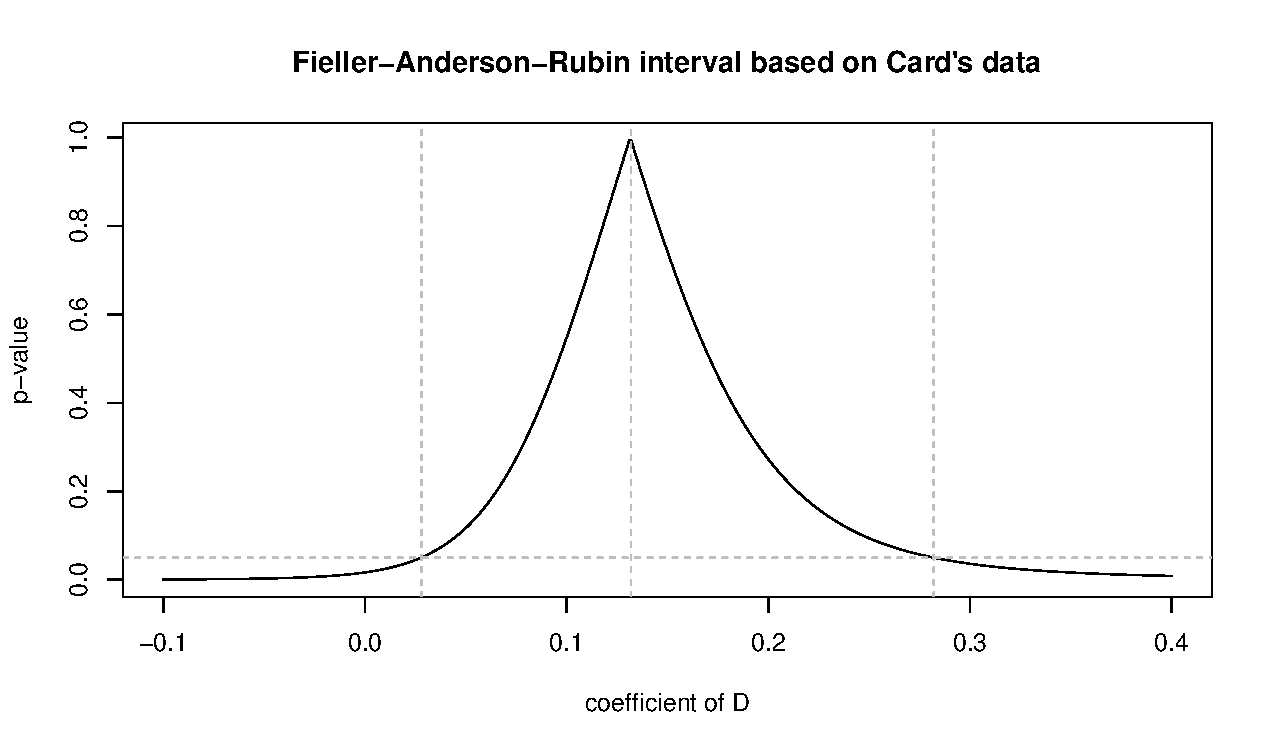
\includegraphics[width = \textwidth]{figures/FAR_Carddata.pdf}
\caption{通过反演检验重新分析\citet{card1993using}的数据} \label{fig::card-far-ci} 
\end{figure}

 
 
 
\section{习题作业}

\paragraph{第\ref{sec::sec::iv-over-identify}节 TSLS 的进一步代数推导}\label{prob::algebra-tsls}

\begin{enumerate}
\item 
证明\eqref{eq::ols-donz}中的$\hat \Gamma$等于
$$
\hat{\Gamma} = \left(  \sumn Z_i Z_i\tran  \right)^{-1} \sumn Z_i D_i\tran .
$$

\item
证明：若$Z$与$D$维数相同，且
$$
n^{-1} \sumn Z_i Z_i\tran, \quad n^{-1} \sumn Z_i D_i\tran
$$
均可逆，则\eqref{eq::2sls-definition}定义的$\hat{\beta}_\textsc{tsls} $退化为\eqref{eq::iv-estimator}定义的$ \hat{\beta}_\textsc{iv}$。 
\end{enumerate}

\paragraph{间接法等价性证明}\label{para::tsls-ils}
证明定理 \ref{thm::ils=2sls}。 


注：使用第\ref{appendix::basic-linear-regression}章的 FWL 定理。 



\paragraph{线性工具变量模型中的控制函数}\label{para::control-function-iv}

下面的定义 \ref{def::cf} 与上面的定义 \ref{def::2sls} 相对应。

\begin{definition}
[探讨第三种估计思路的适用性。]\label{def::cf}
将控制函数估计量$\hat{\beta}_\textsc{cf}$定义如下。
\begin{enumerate}
\item
将$D$对$Z$作 OLS 回归，得到残差$\check D_i\ (i=1,\ldots, n)$。若$D_i$为向量，则逐分量回归，得到$\check D_i$。将残差向量按行$\check{D}_i\tran $组成矩阵$\check{D}$；
\item
将$Y$对$D$和$\check{D}$作 OLS 回归，取$D$的系数为$\hat{\beta}_\textsc{cf}$。  
\end{enumerate}
\end{definition}
 
 证明 $\hat{\beta}_\textsc{cf} = \hat{\beta}_\textsc{tsls}$。
 
 
 注：可利用习题\ref{hw::ols-orthogonal}与\ref{hw::ols-transform-regressors}证明。在定义\ref{def::cf}中，第一步得到的$\check{D}$称为第二步的控制函数。\citet{hausman1978specification}指出了这一结果，\citet{wooldridge2015control}则更一般地讨论了复杂模型中的控制函数方法。 
 
  


 

%\paragraph{Data analysis: \citet{card1993using}}
%
%\citet{card1993using} used the geographic variation in college proximity to estimate the return to schooling. The treatment is education and the outcome is log wage. The IV is the college proximity. 
%\texttt{card.csv} is a slightly modified version of the data from Card's homepage with detailed explanations of the variable names in \texttt{code\_bk.txt}.
%
%You can dichotomize the education variable and infer the LATE. How do you choose the threshold for the dichotomization? Are the results sensitive to your choice? Conduct an analysis with covariates. 
%
%Without dichotomizing the education variable, you can use the standard two-stage least squares estimator. Compare the results to the above analysis.
%
%What if the return of education is nonlinear? Do the data provide information for us to test the nonlinearity?
%


\paragraph{数据分析：\citet{efron1991compliance}}

\citet{efron1991compliance}是较早用潜在结果框架处理不依从的研究之一。原始随机实验“脂质研究诊所冠心病一级预防试验”（LRC-CPPT）旨在评价考来烯胺对胆固醇水平的效应。\texttt{EF.csv}数据第一列为处理／对照二元指标，第二列为实际服用量占名义剂量的比例，最后三列为胆固醇水平。受试者不知道自己被分到药物还是安慰剂，但副作用差异可能使依从行为随分组而不同。所有人被指定相同名义剂量，并服用相同时间。第 3 列$C_3$测于告知低胆固醇饮食益处之前；第 4 列$C_4,$测于饮食建议之后、药物或安慰剂随机分配之前；第 5 列$C_5$为随机分配后胆固醇读数的均值，每两个月测量一次，受试者的随访时间平均为 7.3 年。\citet{efron1991compliance}以胆固醇变化$C_5 - 0.25C_3 - 0.75C_4$为最终结果，原论文有更详细说明。 
 

这里的数据结构比第\ref{chapter::iv-experiment}、\ref{chapter::iv-inequalities}章的不依从问题更复杂。\citet{jin2008principal}基于后文第\ref{chapter::principal-stratification}章的思想重新分析了数据。可按自己对问题的理解选择分析方法，但需说明选择依据。本题没有公认的标准答案。 




 \paragraph{推荐阅读}


\citet{imbens2014instrumental}介绍了计量经济学家的工具变量视角。 

